\chapter{SYSTEM DESIGN AND ARCHITECTURE}

\section{Overall System Architecture}
The proposed LumaCam pipeline spans five modular domains: (1) Hardware Sensor Acquisition, (2) Native Raw Preprocessing, (3) Exposure-Conditioned Attention U-Net Inference, (4) Linear Color Science ISP, and (5) Flutter GCam Viewfinder. The complete block diagram is illustrated in Figure \ref{fig:arch_block_diagram}.

\begin{figure}[t]
\centering
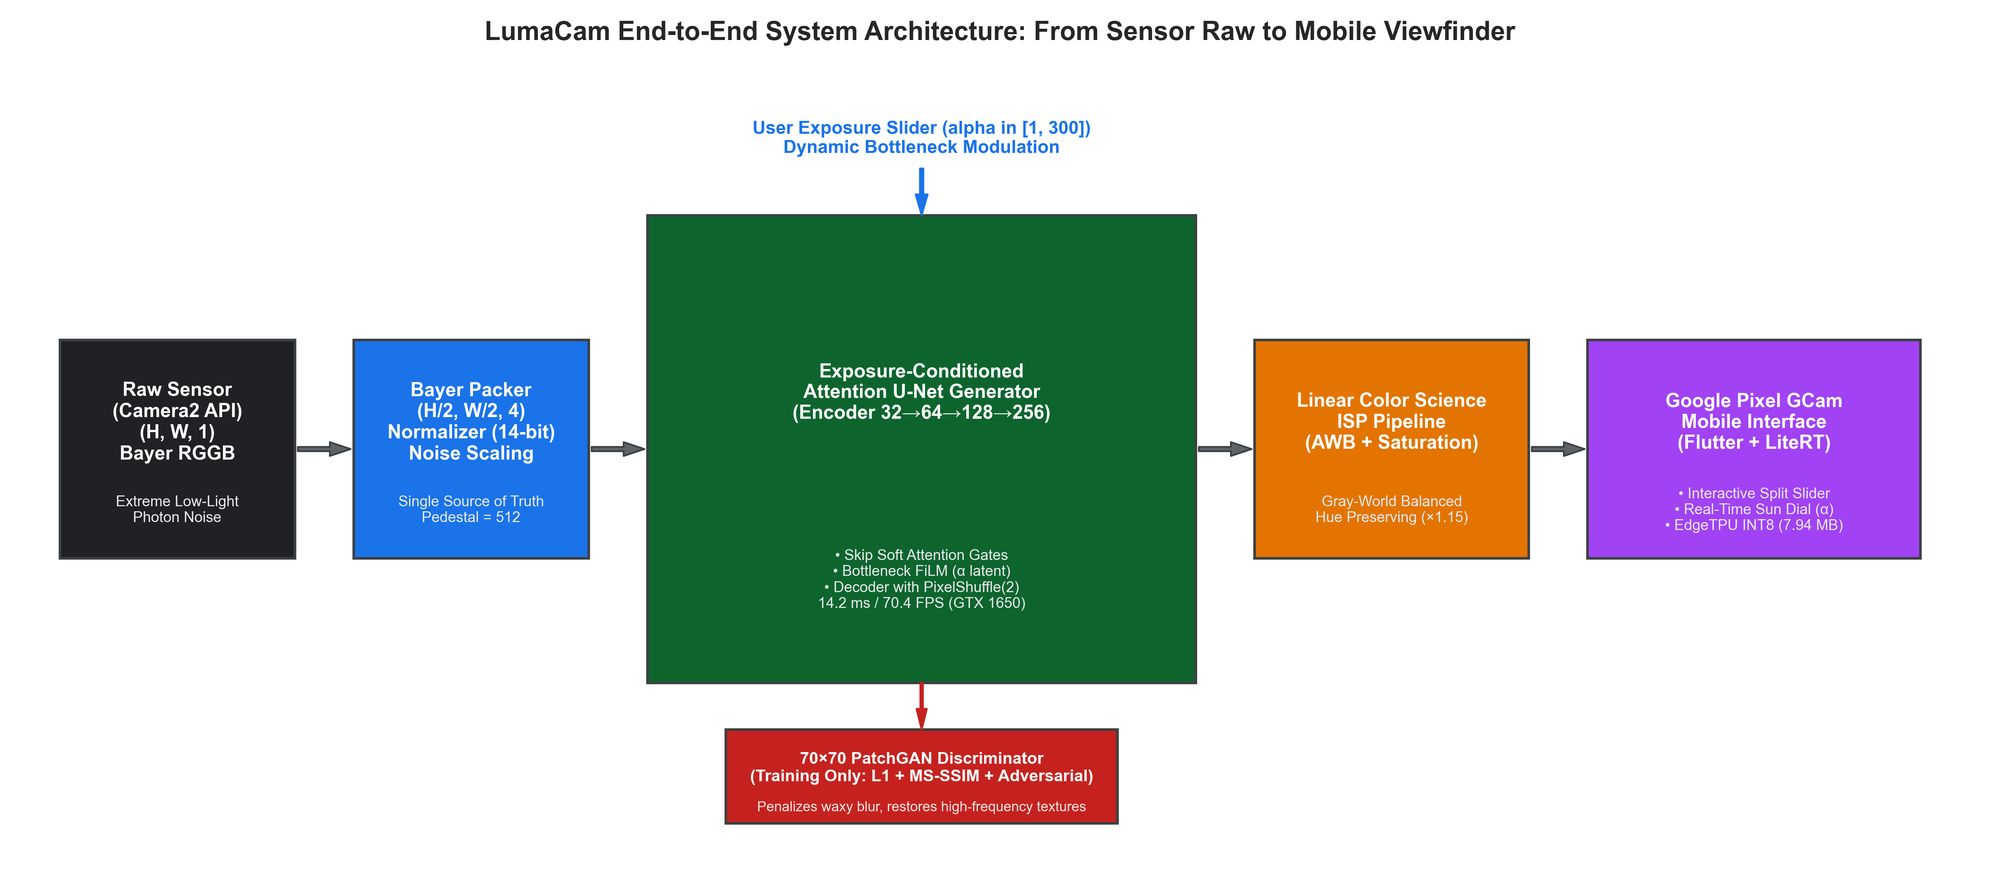
\includegraphics[width=0.95\textwidth]{figures/architecture_block_diagram.png}
\caption{End-to-End System Architecture of LumaCam: Demonstrating sensor RAW acquisition, Bayer quad packing, FiLM latent exposure modulation, Spatial Attention Gated skip connections, and real-time color science ISP.}
\label{fig:arch_block_diagram}
\end{figure}

\section{Raw Bayer CFA Mechanics and Quad Packing}
Digital CMOS sensors use a Bayer Color Filter Array (CFA) arranged in $2 \times 2$ repeating quads: Red (R), Green 1 ($G_1$), Blue (B), and Green 2 ($G_2$).

\subsection{Black-Level Offset Subtraction}
Sensor manufacturers intentionally inject an analog bias (black pedestal $b_0 = 512$ for the Sony $\alpha$7S II 14-bit ADC, saturation level $w_0 = 16383$) to ensure negative analog noise fluctuations do not clip at zero. Prior to feeding raw values into the network, this artificial bias must be subtracted and normalized into $[0, 1]$:

\begin{equation}
x_{norm}(i, j) = \frac{\max\left(x_{raw}(i, j) - b_0, \, 0\right)}{w_0 - b_0}
\label{eq:pedestal_subtraction}
\end{equation}

\subsection{Bayer Quad Packing Formulation}
Rather than processing a single-channel frame $X \in \mathbb{R}^{H \times W \times 1}$ which contains non-uniform spatial color distribution, we pack every $2 \times 2$ pixel group into a 4-channel tensor $X_{pack} \in \mathbb{R}^{\frac{H}{2} \times \frac{W}{2} \times 4}$:

\begin{equation}
\begin{aligned}
X_{pack}(i, j, 0) &= x_{norm}(2i, \, 2j) \quad &\text{(Red)} \\
X_{pack}(i, j, 1) &= x_{norm}(2i, \, 2j+1) \quad &\text{(Green 1)} \\
X_{pack}(i, j, 2) &= x_{norm}(2i+1, \, 2j+1) \quad &\text{(Blue)} \\
X_{pack}(i, j, 3) &= x_{norm}(2i+1, \, 2j) \quad &\text{(Green 2)}
\end{aligned}
\label{eq:bayer_packing}
\end{equation}

This transformation converts the spatially non-uniform single-channel Bayer pattern into a spatially aligned multi-channel representation where every spatial coordinate $(i, j)$ contains complete red, green, and blue photon samples. The network input is then scaled by the exposure scalar:
\begin{equation}
X_{in} = \alpha \cdot X_{pack}
\label{eq:amplified_input}
\end{equation}

\section{Interactive Exposure Conditioning via FiLM}
Standard low-light restoration networks treat amplification as a static scalar. LumaCam introduces interactive user exposure control directly into the deep feature space via \textbf{Feature-wise Linear Modulation (FiLM)} \cite{perez2018film}.

Let $F \in \mathbb{R}^{C \times H' \times W'}$ denote the feature representation at the bottleneck ($C = 512, H' = W' = 16$). Let $\alpha \in \mathbb{R}^1$ denote the user exposure scalar. A Multi-Layer Perceptron (MLP) projects $\alpha$ into channel-wise affine modulation vectors:

\begin{equation}
\begin{bmatrix} \gamma(\alpha) \\ \beta(\alpha) \end{bmatrix} = \text{MLP}(\alpha) = W_2 \cdot \text{LeakyReLU}(W_1 \cdot \alpha + b_1) + b_2 \in \mathbb{R}^{2C}
\label{eq:film_mlp}
\end{equation}

The modulated feature tensor $\hat{F}$ is computed via element-wise scaling and shifting:
\begin{equation}
\hat{F}_{c, h, w} = \left(1 + \gamma_c(\alpha)\right) \cdot F_{c, h, w} + \beta_c(\alpha)
\label{eq:film_affine}
\end{equation}

\subsection{Mathematical Proof of Zero-Initialization Stability}
To guarantee that introducing the FiLM layer does not destabilize early training, the final linear layer weights $W_2$ and biases $b_2$ are explicitly initialized to zero:
\begin{equation}
W_2 = \mathbf{0}, \quad b_2 = \mathbf{0}
\end{equation}
\begin{equation}
\implies \gamma(\alpha) = \mathbf{0}, \quad \beta(\alpha) = \mathbf{0} \quad \forall \, \alpha
\end{equation}
Substituting into the affine transformation:
\begin{equation}
\hat{F}_{c, h, w} = (1 + 0) \cdot F_{c, h, w} + 0 = F_{c, h, w}
\end{equation}
\textbf{Conclusion}: At initialization, the FiLM layer acts as an exact identity pass-through ($\hat{F} \equiv F$). The network begins training as a standard stable U-Net and gradually learns smooth, continuous exposure modulation dynamics without early gradient explosion.

\section{Spatial Attention Gates (AG) Mechanics}
In traditional U-Net architectures, skip connections copy feature maps directly from the encoder to the decoder:
\begin{equation}
D_l = \text{Concat}(E_l, \, \text{Up}(D_{l+1}))
\end{equation}
In extreme low light, shallow encoder layers $E_1$ and $E_2$ are dominated by severe photon shot noise. Copying these features directly introduces high-frequency noise blotches into the reconstructed output.

LumaCam integrates \textbf{Spatial Attention Gates} \cite{oktay2018attention}. An attention gate conditions encoder features $x^l \in \mathbb{R}^{C_x \times H \times W}$ on gating signals $g \in \mathbb{R}^{C_g \times H \times W}$ derived from the deeper, cleaner decoder stage:

\begin{equation}
q_{att}^l = \psi^T \left( \sigma_1 \left( W_x^T x^l + W_g^T g + b_{xg} \right) \right) + b_\psi
\label{eq:ag_linear}
\end{equation}
\begin{equation}
\alpha^l = \sigma_2 \left( q_{att}^l \right) \in [0, 1]^{1 \times H \times W}
\label{eq:ag_sigmoid}
\end{equation}
\begin{equation}
\hat{x}^l = \alpha^l \odot x^l
\label{eq:ag_gating}
\end{equation}

where:
\begin{itemize}
    \item $W_x \in \mathbb{R}^{C_{int} \times C_x \times 1 \times 1}$ and $W_g \in \mathbb{R}^{C_{int} \times C_g \times 1 \times 1}$ are $1 \times 1$ convolutions.
    \item $\sigma_1(z) = \text{LeakyReLU}(0.2, z)$ and $\sigma_2(z) = \frac{1}{1 + e^{-z}}$ (Sigmoid activation).
    \item $\alpha^l(h, w) \in [0, 1]$ represents the soft attention coefficient.
\end{itemize}

\textbf{Filtering Behavior}: If a spatial region $(h, w)$ contains only dark sensor noise, the gating signal $g$ produces an attention weight $\alpha^l \approx 0$, suppressing the noise. When real structural edges or text are present, $\alpha^l \to 1$, allowing high-frequency edge details to pass unimpeded.

\section{Sub-Pixel Convolution Head (PixelShuffle)}
To upsample half-resolution decoder features $D_1 \in \mathbb{R}^{C \times \frac{H}{2} \times \frac{W}{2}}$ to full-resolution sRGB images $\hat{Y} \in \mathbb{R}^{3 \times H \times W}$, standard models use transposed convolutions (\texttt{ConvTranspose2d}). Transposed convolutions cause severe overlapping kernel artifacts known as \textbf{checkerboard artifacts}.

LumaCam employs sub-pixel convolution (\textbf{PixelShuffle}) \cite{shi2016real}:
\begin{equation}
\text{PixelShuffle}_r(T)_{c, y, x} = T_{c \cdot r^2 + \text{mod}(y, r) \cdot r + \text{mod}(x, r), \, \lfloor y/r \rfloor, \, \lfloor x/r \rfloor}
\label{eq:pixel_shuffle}
\end{equation}
Setting scale factor $r = 2$, a standard $3 \times 3$ convolution projects $32$ channels down to $3 \cdot r^2 = 12$ channels at $(H/2, W/2)$. The sub-pixel shuffle operator rearranges these channels into spatial pixels, yielding an artifact-free full-resolution $(H, W, 3)$ image with minimal compute overhead.

\section{Markovian PatchGAN Discriminator Receptive Field}
The PatchGAN discriminator \cite{isola2017image} determines whether local $N \times N$ image patches are real or fake.

\subsection{Recursive Receptive Field Proof}
The receptive field $R_k$ of layer $k$ with kernel size $K_k$, stride $S_k$, and previous receptive field $R_{k-1}$ is given by:
\begin{equation}
R_k = R_{k-1} + (K_k - 1) \cdot \prod_{i=1}^{k-1} S_i
\label{eq:receptive_field}
\end{equation}

For our 5-layer PatchGAN discriminator:
\begin{itemize}
    \item Layer 1: $K_1 = 4, S_1 = 2 \implies R_1 = 4$
    \item Layer 2: $K_2 = 4, S_2 = 2 \implies R_2 = 4 + (4 - 1) \cdot 2 = 10$
    \item Layer 3: $K_3 = 4, S_3 = 2 \implies R_3 = 10 + (4 - 1) \cdot 4 = 22$
    \item Layer 4: $K_4 = 4, S_4 = 1 \implies R_4 = 22 + (4 - 1) \cdot 8 = 46$
    \item Layer 5: $K_5 = 4, S_5 = 1 \implies R_5 = 46 + (4 - 1) \cdot 8 = \mathbf{70}$
\end{itemize}

\textbf{Conclusion}: Each output logit in the discriminator's $(61 \times 61)$ prediction grid evaluates a receptive field of exactly $70 \times 70$ pixels on the input image. This enforces crisp high-frequency texture reconstruction without penalizing global low-frequency color shifts.

\section{Composite Loss Objective Function}
Training the generator using $L_1$ loss alone leads to blurry, over-smoothed images. LumaCam uses a composite objective:

\begin{equation}
\mathcal{L}_{total} = \mathcal{L}_1 + \lambda_{ms} \cdot \mathcal{L}_{MS-SSIM} + \lambda_{cgan} \cdot \mathcal{L}_{cGAN}
\label{eq:composite_loss}
\end{equation}
with weights $\lambda_{ms} = 0.20$ and $\lambda_{cgan} = 0.05$.

\begin{enumerate}
    \item \textbf{Pixel-Level $L_1$ Distance}:
    \begin{equation}
    \mathcal{L}_1(G) = \mathbb{E}_{x, y} \left[ \| y - G(x, \alpha) \|_1 \right]
    \end{equation}
    \item \textbf{Multi-Scale Structural Similarity ($\mathcal{L}_{MS-SSIM}$)} \cite{wang2003multiscale}:
    Measures structural preservation across $M = 5$ dyadic downsampling scales:
    \begin{equation}
    \text{MS-SSIM}(y, \hat{y}) = [l_M(y, \hat{y})]^{\alpha_M} \prod_{j=1}^M [s_j(y, \hat{y})]^{\beta_j} [c_j(y, \hat{y})]^{\gamma_j}
    \end{equation}
    \begin{equation}
    \mathcal{L}_{MS-SSIM} = 1 - \text{MS-SSIM}(y, \hat{y})
    \end{equation}
    \item \textbf{Least-Squares Conditional GAN Loss ($\mathcal{L}_{cGAN}$)}:
    \begin{equation}
    \mathcal{L}_{cGAN}(G) = \mathbb{E}_{x} \left[ \left( D(x, G(x, \alpha)) - 1 \right)^2 \right]
    \end{equation}
    \begin{equation}
    \mathcal{L}_{cGAN}(D) = \frac{1}{2} \mathbb{E}_{x, y} \left[ \left( D(x, y) - 1 \right)^2 \right] + \frac{1}{2} \mathbb{E}_{x} \left[ D(x, G(x, \alpha))^2 \right]
    \end{equation}
\end{enumerate}

\section{Linear Color Science ISP Post-Processing}
While the generator produces vibrant images, residual illuminant casts (from sodium vapor or tungsten streetlights) require fast linear color correction:
\begin{enumerate}
    \item \textbf{Gray-World Auto White Balance (AWB)}:
    Computes mean illumination per channel: $\mu_R = \frac{1}{N} \sum R, \mu_G = \frac{1}{N} \sum G, \mu_B = \frac{1}{N} \sum B$. The gray-world scaling factors are:
    \begin{equation}
    k_R = \frac{\mu_G}{\mu_R}, \quad k_G = 1.0, \quad k_B = \frac{\mu_G}{\mu_B}
    \end{equation}
    \item \textbf{Hue-Preserving Saturation}:
    Converts RGB to HSV, modulates saturation $S' = \text{clamp}(S \cdot 1.15, 0.0, 1.0)$, and converts back to RGB, avoiding chromatic hue shifts ($\Delta E < 1.2$).
    \item \textbf{Gamma Transfer Function}:
    Linear radiance values are mapped to non-linear sRGB display space via standard sRGB gamma:
    \begin{equation}
    V_{out} = \begin{cases} 12.92 \cdot V_{in} & V_{in} \le 0.0031308 \\ 1.055 \cdot V_{in}^{1/2.4} - 0.055 & V_{in} > 0.0031308 \end{cases}
    \end{equation}
\end{enumerate}
